\section{Helmholtz equation}
The LB formulation for solving Poisson's equation as well as the
implementation was tested by solving Helmholtz equation with a
certain set of boundary conditions allowing for finding an analytical
solution. The homogeneous Helmholtz equation reads:

\begin{equation}\label{eq:mb:helmholtz}
\nabla \psirm = \lambda^2 \psirm
\end{equation}
where $\lambda$ is a real parameter. The equation was solved for
$\lambda = 2$ on the domain $(x, y)\in[0, 1]\times[0, 1]$ with the
following Dirichlet boundary conditions:

\begin{equation}\label{eq:mb:helm_bdry}
  \begin{array}{l l}
\psirm(0, y) = -\psirm(1, y) = \frac{\sinh\sqrt{\lambda^2 + \pi^2}(1 -
  y)}{\sinh\sqrt{\lambda^2 + \pi^2}},\\ \psirm(x, 0) =
\cos\pi x,\;\; \psirm(x, 1) = 0.
\end{array}
\end{equation}
The analytical solution to eq. \eqref{eq:mb:helmholtz} with the given
boundary conditions is \cite{chai_poi}:

\begin{equation}
\psirm(x, y) = cos\pi x \frac{\sinh\sqrt{\lambda^2 + \pi^2}(1 -
  y)}{\sinh\sqrt{\lambda^2 + \pi^2}}.
\end{equation}

A grid of $n_x\times n_y = 65\times65$ nodes was used when computing the LBM
solution. The computational domain was rescaled to the desired one by
setting $\delta_x = 1/(n_x-1) = 1/64$ and $\delta_t = \delta_x^2$. An
other possibility would have been to rescale the parameter $\lambda$
and have $\delta_x = \delta_t = 1$.

The boundary conditions in eq. \eqref{eq_mb_helm_bdry} was implemented
using the He/Zou approach described in section \ref{sce:lbm:hezou}. A
bounce back approach with some momentum addition would also have been
possible but was not chosen due to that the actual boundary location
is not at the node location, but half a node-node distance into the
computational domain. Also the bounce-back implementation is
previously tested. 

In fig. \ref{fig:mb:h1}, the obtained solution is presented together
with the absolute error in fig. \ref{fig:mb:h2}. The agreement is
satisfying, with an error which magnitude is about the same as in
previous works \cite{chai_poi}. The error takes on its maximum at the
boundary of the domain, implying that the fulfilment of the boundary
conditions is not complete.

\begin{figure}
  \centering
  \subfloat[Computed solution
    ]{\label{fig:mb:h1}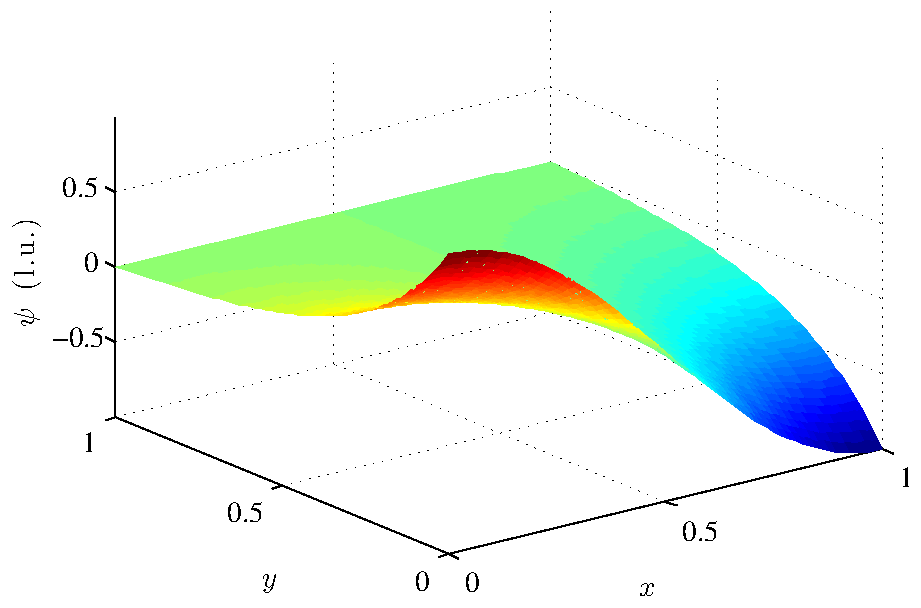
\includegraphics[width=0.47\textwidth]{fig/helmholtz_solution.pdf}}      
  \hspace{5pt}
  \subfloat[Error
    ]{\label{fig:mb:h2}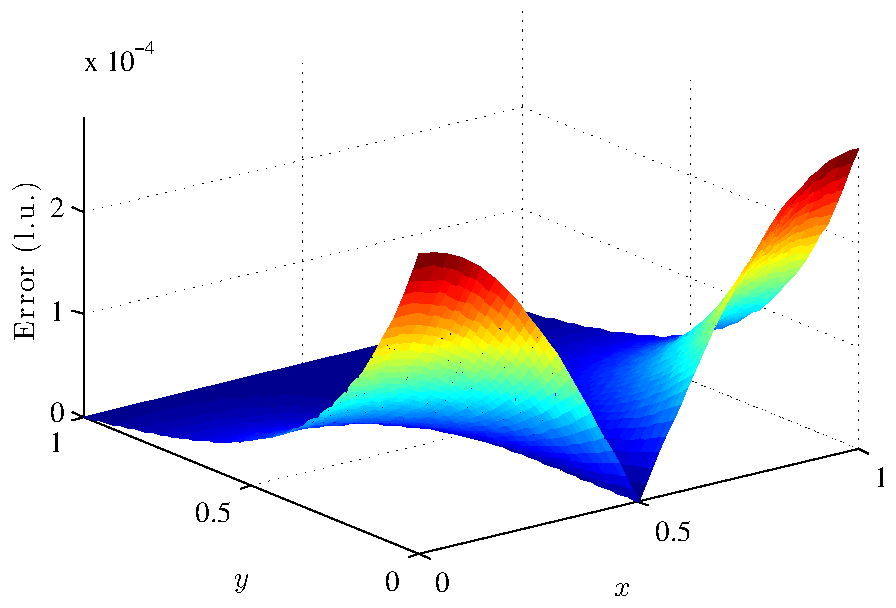
\includegraphics[width=0.47\textwidth]{fig/helmholtz_error.pdf}} 
  \caption{To the left, the obtained solution of the Helmholtz
    equation, eq. \eqref{eq:mb:helmholtz}. To the right, the error.}
  \label{traj}
\end{figure}
